\subsection{История разработки промышленных протоколов}
\subsubsection{Предыстория появления автоматизации}
Автоматизация подразумевает в себе соединение воедино различного оборудования. С развитием промышленности требования всё возрастали, что создало спрос на различного вида интерфейсы между измерительным прибором или устройством с системой измерения и управления. К тому же появилась необходимость записи полученных данных \cite{van_gorp_advanced_2009}. 


В течение многих лет системы обмена данными строились вокруг одного мощного вычислительного устройства, к которому шло огромное количество кабелей. Подобная структура была дорога в обслуживании и отличалась низкой степенью автоматизации. 

Альтернативой стали так называемые ЦПС, которые состоят из узлов, обменивающихся данными цифровым способом. На сегодняшний момент таких систем насчитывается большое количество \cite{__2002}.

Уже более 30 лет широко применяется слово \fb. Обычно под этим термином понимается сеть, которая соединяет различного рода устройства (ПЛК, сенсоры) с человеко - машинным интерфейсом (MMI). В это понятие входит множество протоколов, разнообразие которых обусловлено \cite{thomesse_fieldbus_2005}:
\begin{itemize}
	\item нуждой разнообразных компаний из разных областей в средстве сбора и обмена данными в промышленных сетях;
	\item огромному числу разнообразных сенсоров, датчиков и устройств, которые необходимо  было соединить между собой.
\end{itemize}
\subsubsection{Технология Fieldbus: возникновение и требования}
Есть несколько причин возникновения концепта \fb, но их можно разделить на 2 основные группы \cite{thomesse_fieldbus_2005}:
\begin{enumerate}
	\item Потребности пользователей (предприятий):
	\begin{enumerate}
		\item Необходимость единого стандарта;
		\item Концепт предприятия, управляемого компьютерами.
	\end{enumerate}
	\item Возможности технологий:
	\begin{enumerate}
		\item Модель OSI (см. \refris{fig:osi})
		\item Возможности микроэлектроники (внедрение ``интеллекта'' даже в маленькие датчики, ``распределённый интеллект'').
	\end{enumerate}
\end{enumerate}

Последующее развитие индустрии показало, что пользователи выбирают открытые протоколы, поскольку в отличие от проприетарных решений они обладают следующими преимуществами \cite{galloway_introduction_2012}:
\begin{itemize}
	\item большее число поддерживаемого оборудования;
	\item возможность разделить стоимость разработки протокола между компаниями, которые готовы вкладываться в разработку свободного ПО;
	\item качество поддержки открытого ПО обычно выше, чем у проприетарного.
\end{itemize}
\subsubsection{Modbus}
Протокол \mb{} RTU был разработан компанией Modicon (в настоящее время - Schneider Electric) в 1979 году для использования в ПЛК собственного производства. На текущий момент является де - факто стандартом для связи устройств промышленной сети \cite{__2001, van_gorp_advanced_2009}. 

Изначально протокол работал по интерфейсу RS-232, позднее появилась реализации протокола для интерфейсов RS-485 и TCP. Протокол быстро набрал популярность, и многие производители стали внедрять его в своих устройствах.

Позже права на протокол были переданы некоммерческой организации Modbus Organization, которая до сегодняшнего дня владеет стандартом \cite{advantech__2019}.

По распространённости в России конкурирует только с \pb \cite{__2010}. 
\subsubsection{Profibus}
Если протокол \mb{} можно назвать ``дедушкой'' протоколов, то \pb -- ``молодой атлет'': худой и быстрый. Он был разработан в 90-х годах прошлого века для удовлетворения всех потребностей промышленной связи
как для автоматизации производства, так и для автоматизации процессов \cite{powell_profibus_2013}.

\pb настроен как универсальная и открытая (открыт не до конца \cite{__2001}) система связи. Первоначально разработанный для обеспечения дискретного производства, он расширился до автоматизации процессов и корпоративных приложений. \pb включает в себя несколько спецификаций протокола промышленной шины, включая \cite{van_gorp_advanced_2009}:
\begin{itemize}
	\item \textit{Profibus-DP};
	\item \textit{Profibus-PA};
	\item \textit{PROFInet} и другие.
\end{itemize}

Разработавшая его компания Siemens AG до сих пор является основным разработчиком вариаций данной платформы. Несмотря на то, что стандарт позиционируется как открытый, открытыми являются только нижние уровни сетевого взаимодействия. Протоколы доступа к среде, форматы кадров, интерфейсы взаимодействия с приложени­ями прикладного уровня регламентируются проприетарными прото­колами фирмы Siemens. Для получения доступа к ним требуется всту­пление в группу разработчиков стандарта \pb \cite{__2001}.

\subsubsection{Foundation Fieldbus}
\ffb является цифровой системой связи, применяемой в автоматизациии наряду с такими, как \pb и \mb. В настоящий момент включает в себя два протокола информационного обмена между участниками сети \cite{phoenix_contact__2020}: 
\begin{itemize}
	\item H1;
	\item HSE.
\end{itemize}

Стандарт был разработан \textit{American Fieldbus Foundation} в ответ на задержки по созданию международного стандарта \fb \cite{galloway_introduction_2012}. 

Изначально разработанный для решений низкоуровневых задач автоматизации протокол \fb теперь носит название \textit{Fieldbus H1} в связи с появлением таких решений, как:
\begin{itemize}
	\item \textit{Foundation Fieldbus Safety Instrumented Functions} для использования в местах, где необходима безопасность;
	\item\textit{Foundation Fieldbus \Gls{hse}} для работы на высоких скоростях.
\end{itemize}
\subsection{Принципы работы протоколов}
\subsubsection{Понимание термина Fieldbus}\label{par:fieldbus}
В дословном переводе термин \fb означает ``промышленная сеть'', однако это не определённый протокол передачи данных и не тип архитектуры. Под этим термином лучше всего представить сферу применения. 

Промышленная сеть -- это \cite{__2001}:
\begin{itemize}
	\item среда передачи данных, отвечающая жёстким и, зачастую, противоречивым требованиям;
	\item набор стандартных протоколов обмена данными, позволяющих связать воедино оборудование различных производителей, а также обеспечить взаимодействие нижнего и верхнего уровней
\end{itemize}

Обычно \fb -- это двунаправленная цифровая сеть, используемая для контроля и автоматизации. Сеть состоит из \cite{van_gorp_advanced_2009}:
\begin{itemize}
	\item человеко - машинный интерфейс;
	\item главная контролирующая система (master);
	\item набор интерфейсов (slave) между датчиками, насосами, и прочим оборудованием. 
\end{itemize}

Использование подобной системы способно уменьшить время простоя, заранее сообщая диагностические данные оператору. 
\subsubsection{Принцип работы промышленной сети}
\paragraph{Принцип работы промышленной автоматики}
В процессе автоматизации всё делится на 2 уровня. Пример построения такой системы показан на \refris{fig:topology} \cite{promwad__2019}:
\begin{itemize}
	\item \textbf{нижний:} уровень связи устройств управления и подведомственного оборудования (их ещё называют полевые устройства);
	\item \textbf{верхний:} панель управления оператора, через которую он может отслеживать происходящее на объекте автоматизации. Именно на верхнем уровне располагается система управления и автоматизации SCADA \newline (см. \refpar{par:scada}). 
\end{itemize}
\begin{figure}[H]
	\centering
	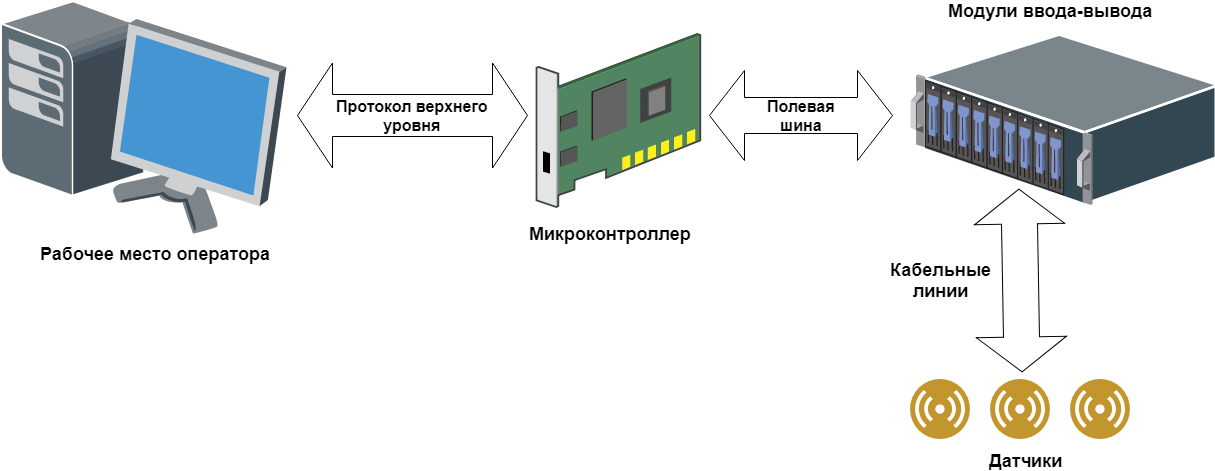
\includegraphics[width=0.9\linewidth]{images/topology}
	\caption{Общая схема автоматизации объекта}
	\label{fig:topology}
\end{figure}
\paragraph{Топология сети}\label{par:topology}
Существует три наиболее значимых топологии сети автоматизации \cite{__2001}. 
\begin{enumerate}
	\item \textbf{Общая шина.} Структура топологии приведена на \refris{fig:shina}.
	\begin{itemize}
		\item \textbf{Достоинства:}
		\begin{itemize}
			\item простая;
			\item недорогая;
			\item лёгкая в настройке;
			\item хорошо подходит для сильно распределённых объектов.
		\end{itemize}
		\item \textbf{Недостатки:}
		\begin{itemize}
			\item присутствие в каждой точке сети общего трафика;
			\item потеря связи при одиночном обрыве канала.
		\end{itemize}
	\end{itemize}
	\begin{figure}
		\centering
		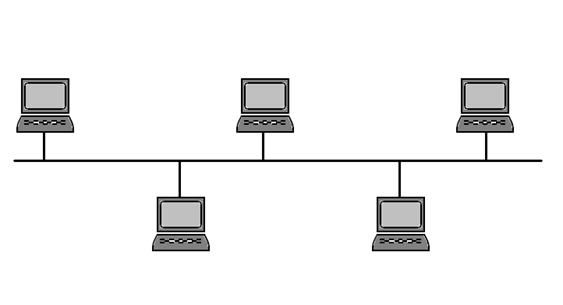
\includegraphics[width=0.5\linewidth]{images/shina}
		\caption{Топология ``общая шина''}
		\label{fig:shina}
	\end{figure}
	\item \textbf{Кольцо.} Структура топологии приведена на \refris{fig:kolco}.
	\begin{itemize}
		\item \textbf{Достоинства:}
		\begin{itemize}
			\item абсолютная предсказуемость трафика;
			\item хорошая пропускная способность.
		\end{itemize}
		\item \textbf{Недостатки:}
		\begin{itemize}
			\item высокая стоимость организации канала связи;
			\item нерациональное использование сетевого трафика при неправильной конфигурации;
			\item потеря всей синхронизации при отключении хотя бы одного из узлов.
		\end{itemize}
	\end{itemize}
	\begin{figure}
		\centering
		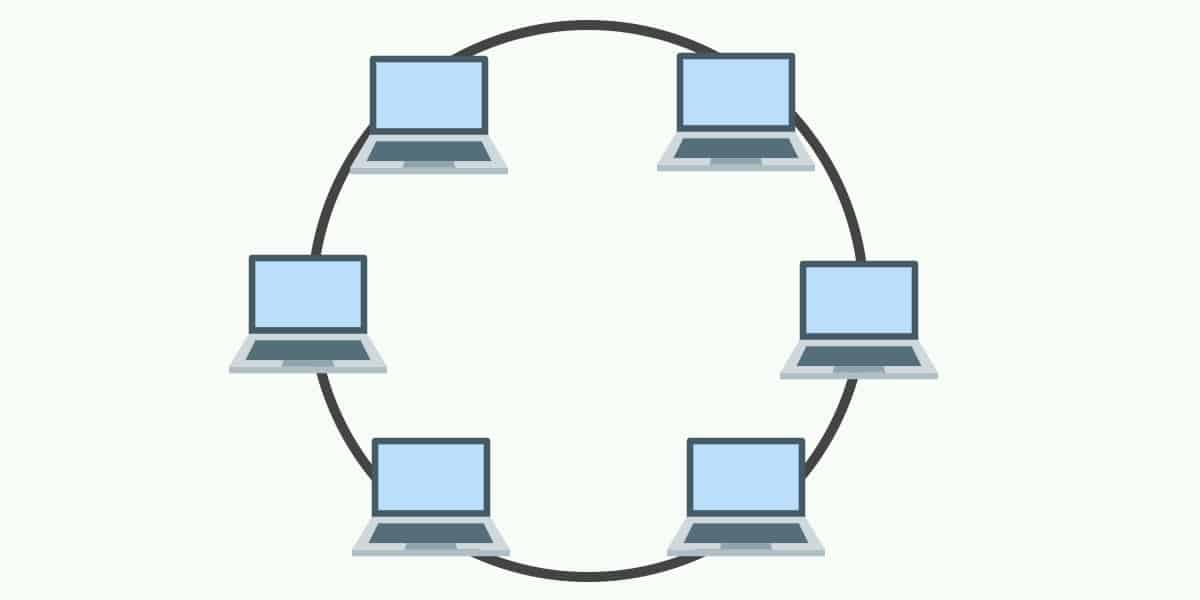
\includegraphics[width=0.5\linewidth]{images/kolco}
		\caption{Топология ``кольцо''}
		\label{fig:kolco}
	\end{figure}
	\item \textbf{Звезда.} Обычно является частью большей сети. Структура топологии приведена на \refris{fig:zvezda}.
	\begin{itemize}
		\item \textbf{Достоинства:}
		\begin{itemize}
			\item дополнительная защита сети от выходи из строя или отключения узлов;
			\item простая масштабируемость;
			\item оптимизация трафика;
			\item допускаются коллизии.
		\end{itemize}
		\item \textbf{Недостатки:}
		\begin{itemize}
			\item обмен идёт через один высоконагруженный компьютер;
			\item потеря связи при одиночном обрыве канала;
			\item ограничение числа рабочих станций числом портов центрального компьютера.
		\end{itemize}
	\end{itemize}
	\begin{figure}
		\centering
		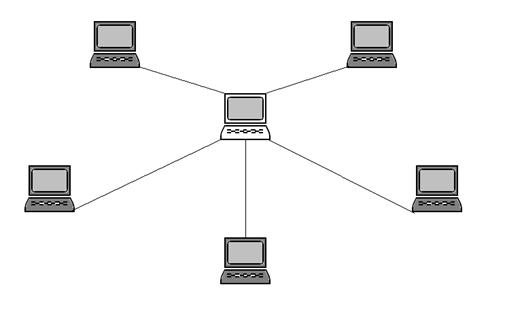
\includegraphics[width=0.5\linewidth]{images/zvezda}
		\caption{Топология ``звезда''}
		\label{fig:zvezda}
	\end{figure}
\end{enumerate}
\paragraph{Основные характеристики сетей}
С развитием техники стало возможным наделить ``интеллектом'' каждый из полевых датчиков. Каждый из узлов цепи способен \cite{__2002}:
\begin{itemize}
	\item принимать команды от других узлов сети;
	\item считывать данные с подключенных датчиков;
	\item оцифровывать полученные данные в случае их представления аналоговым способом;
	\item передавать информацию другим узлам сети.
\end{itemize}
\paragraph{Режимы обмена данными}
В промышленной автоматизации существует три режима обмена данными \cite{__2002, thomesse_fieldbus_2005}:
\begin{enumerate}
	\item \textbf{Ведущий - ведомый.} Ведущее устройство последовательно опрашивает подчинённые узлы. В зависимости от запроса ведомый узел может:
	\begin{itemize}
		\item выполнить полученную команду;
		\item передать ведущему устройству данные с подключенных к нему датчиков.
	\end{itemize}
	Примером таких сетей могуть быть \mb{} и \pb.
	\item \textbf{Клиент - сервер.} Очень похож на предыдущий тип. Клиент запрашивает данные, а сервер их предоставляет. Функции клиента и сервера могуть быть исполнены одним устройством. Отличие от предыдущего пункта -- в отличие от топологии master-slave, топология client-server позволяет серверу автоматически отправлять данные (ведомые устройства этого сделать не могут). Представитель --  \ffb.
	\item \textbf{Подписка.} Узел, нуждающийся в периодическом поступлении информации, подписывается на получение её от другого узла и получает регулярную рассылку без дополнительных запросов. Есть два режима работы:
	\begin{enumerate}
		\item Данные передаются циклически, с определённым интервалом;
		\item Данные передаются только в случае их изменения.
	\end{enumerate}
	Примером такой сети также может быть \ffb.
\end{enumerate}